%
% Masterarbeit von Marcel Weber und Silvio Wangler
% 
% 
\chapter{Methodologie}
%% todo: Methodologie schreiben. (Richtlinie 20 Seiten)
% Im Abschnit Methodologie beschreiben Sie detailliert, wie Sie die praktische / empirische Analyse des Ph�nomens durchgef�hrt
% haben, welches Design (Typ der Arbeit) Sie weshalb gew�hlt, welche qualitativen oder quantitativen Methoden Sie wie eingesetzt
% und wie Sie die gemachten Erkenntnisse gewonnen und daraus Handlungsempfehlungen abgeleitet haben.
%
% Tipp: St�tzen Sie sich bei der Wahl und Anwendung von Methoden auf die entsprechende Literatur.



Die Datenerhebung erfolgt quantitativ (konfirmatorisch) und verfolgt ein nicht experimentelles Erhebungsdesgin in Form zweier Fragebogen (im weiteren Survey genannt). Diese stehen f�r die Probanden dieser Masterarbeit online zur Verf�gung.

\paragraph{}Im Rahmen dieser Masterarbeit wollen wir sowohl von Arbeitgeber als auch von Arbeitnehmer eine Datenerhebung durchf�hren. Die so gewonnen Daten sollen uns f�r einen Ansichtenvergleich der beiden Parteien dienen, mit welchen wir unsere Hypothesen best�tigen bzw. verwerfen wollen. Der Vergleich zwischen Arbeitnehmer und Arbeitgeber wollen wir �ber die Parameter Unternehmensgr�sse und Firmensitz herstellen. D.h. dass alle Probanden die beiden Informationen in dem jeweiligen Survey angeben m�ssen.

\paragraph{}Um zu gew�hrleisten, dass die beiden Surveys repr�sentativ ausfallen, werden die Teilnehmer nach folgenden Kriterien kategorisiert.

\begin{figure}[ht]
	\centering
		
	\ifpdf
		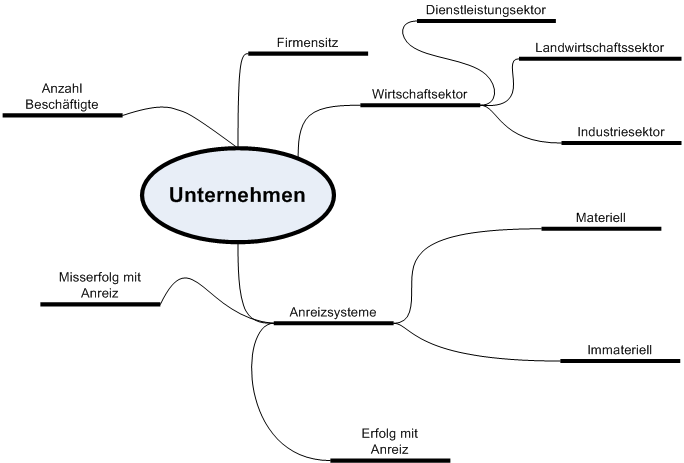
\includegraphics[width=0.8\textwidth]{chap04-MindMap-Survey-Arbeitgeber.png}
	\else	
		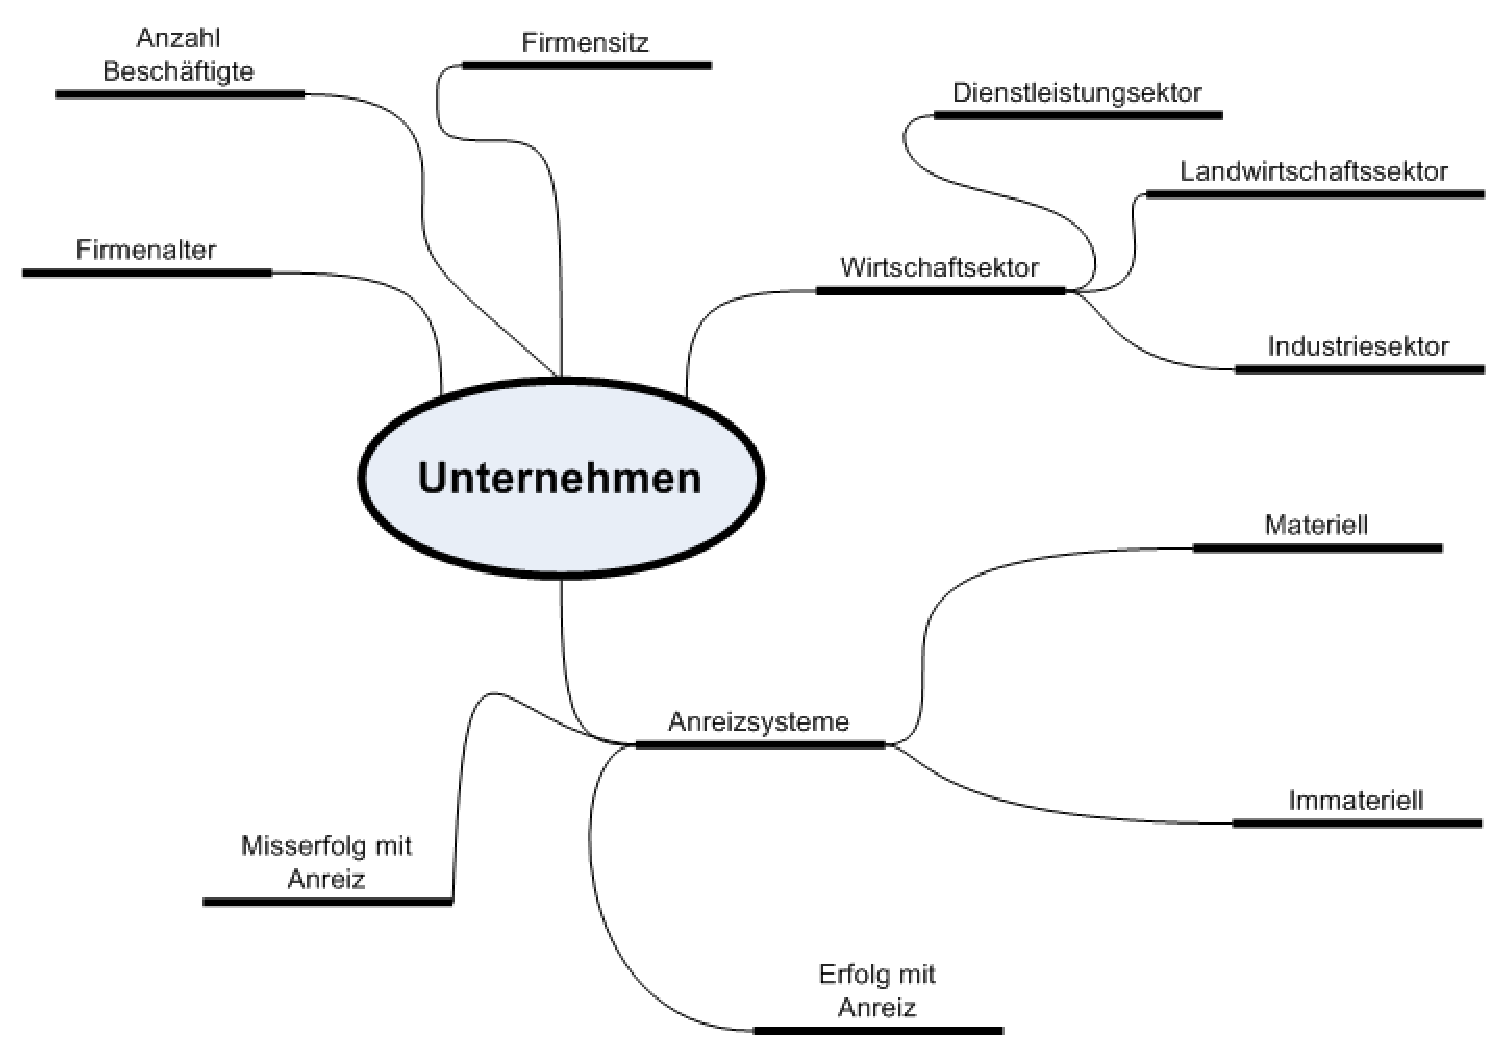
\includegraphics[width=0.8\textwidth]{chap04-MindMap-Survey-Arbeitgeber.eps}
	\fi
		
	\caption[Mindmap Survey Arbeitgeber]{Mindmap Survey Arbeitgeber (Eigene Darstellung)}	
	\label{fig:surveyCompany}
\end{figure}
